\documentclass[1p]{elsarticle_modified}
%\bibliographystyle{elsarticle-num}

%\usepackage[colorlinks]{hyperref}
%\usepackage{abbrmath_seonhwa} %\Abb, \Ascr, \Acal ,\Abf, \Afrak
\usepackage{amsfonts}
\usepackage{amssymb}
\usepackage{amsmath}
\usepackage{amsthm}
\usepackage{scalefnt}
\usepackage{amsbsy}
\usepackage{kotex}
\usepackage{caption}
\usepackage{subfig}
\usepackage{color}
\usepackage{graphicx}
\usepackage{xcolor} %% white, black, red, green, blue, cyan, magenta, yellow
\usepackage{float}
\usepackage{setspace}
\usepackage{hyperref}

\usepackage{tikz}
\usetikzlibrary{arrows}

\usepackage{multirow}
\usepackage{array} % fixed length table
\usepackage{hhline}

%%%%%%%%%%%%%%%%%%%%%
\makeatletter
\renewcommand*\env@matrix[1][\arraystretch]{%
	\edef\arraystretch{#1}%
	\hskip -\arraycolsep
	\let\@ifnextchar\new@ifnextchar
	\array{*\c@MaxMatrixCols c}}
\makeatother %https://tex.stackexchange.com/questions/14071/how-can-i-increase-the-line-spacing-in-a-matrix
%%%%%%%%%%%%%%%

\usepackage[normalem]{ulem}

\newcommand{\msout}[1]{\ifmmode\text{\sout{\ensuremath{#1}}}\else\sout{#1}\fi}
%SOURCE: \msout is \stkout macro in https://tex.stackexchange.com/questions/20609/strikeout-in-math-mode

\newcommand{\cancel}[1]{
	\ifmmode
	{\color{red}\msout{#1}}
	\else
	{\color{red}\sout{#1}}
	\fi
}

\newcommand{\add}[1]{
	{\color{blue}\uwave{#1}}
}

\newcommand{\replace}[2]{
	\ifmmode
	{\color{red}\msout{#1}}{\color{blue}\uwave{#2}}
	\else
	{\color{red}\sout{#1}}{\color{blue}\uwave{#2}}
	\fi
}

\newcommand{\Sol}{\mathcal{S}} %segment
\newcommand{\D}{D} %diagram
\newcommand{\A}{\mathcal{A}} %arc


%%%%%%%%%%%%%%%%%%%%%%%%%%%%%5 test

\def\sl{\operatorname{\textup{SL}}(2,\Cbb)}
\def\psl{\operatorname{\textup{PSL}}(2,\Cbb)}
\def\quan{\mkern 1mu \triangleright \mkern 1mu}

\theoremstyle{definition}
\newtheorem{thm}{Theorem}[section]
\newtheorem{prop}[thm]{Proposition}
\newtheorem{lem}[thm]{Lemma}
\newtheorem{ques}[thm]{Question}
\newtheorem{cor}[thm]{Corollary}
\newtheorem{defn}[thm]{Definition}
\newtheorem{exam}[thm]{Example}
\newtheorem{rmk}[thm]{Remark}
\newtheorem{alg}[thm]{Algorithm}

\newcommand{\I}{\sqrt{-1}}
\begin{document}

%\begin{frontmatter}
%
%\title{Boundary parabolic representations of knots up to 8 crossings}
%
%%% Group authors per affiliation:
%\author{Yunhi Cho} 
%\address{Department of Mathematics, University of Seoul, Seoul, Korea}
%\ead{yhcho@uos.ac.kr}
%
%
%\author{Seonhwa Kim} %\fnref{s_kim}}
%\address{Center for Geometry and Physics, Institute for Basic Science, Pohang, 37673, Korea}
%\ead{ryeona17@ibs.re.kr}
%
%\author{Hyuk Kim}
%\address{Department of Mathematical Sciences, Seoul National University, Seoul 08826, Korea}
%\ead{hyukkim@snu.ac.kr}
%
%\author{Seokbeom Yoon}
%\address{Department of Mathematical Sciences, Seoul National University, Seoul, 08826,  Korea}
%\ead{sbyoon15@snu.ac.kr}
%
%\begin{abstract}
%We find all boundary parabolic representation of knots up to 8 crossings.
%
%\end{abstract}
%\begin{keyword}
%    \MSC[2010] 57M25 
%\end{keyword}
%
%\end{frontmatter}

%\linenumbers
%\tableofcontents
%
\newcommand\colored[1]{\textcolor{white}{\rule[-0.35ex]{0.8em}{1.4ex}}\kern-0.8em\color{red} #1}%
%\newcommand\colored[1]{\textcolor{white}{ #1}\kern-2.17ex	\textcolor{white}{ #1}\kern-1.81ex	\textcolor{white}{ #1}\kern-2.15ex\color{red}#1	}

{\Large $\underline{12n_{0376}~(K12n_{0376})}$}

\setlength{\tabcolsep}{10pt}
\renewcommand{\arraystretch}{1.6}
\vspace{1cm}\begin{tabular}{m{100pt}>{\centering\arraybackslash}m{274pt}}
\multirow{5}{120pt}{
	\centering
	\includegraphics[width=112pt]{../../../GIT/diagram.site/Diagrams/png/2465_12n_0376.png}\\
\ \ \ A knot diagram\footnotemark}&
\allowdisplaybreaks
\textbf{Linearized knot diagam} \\
\cline{2-2}
 &
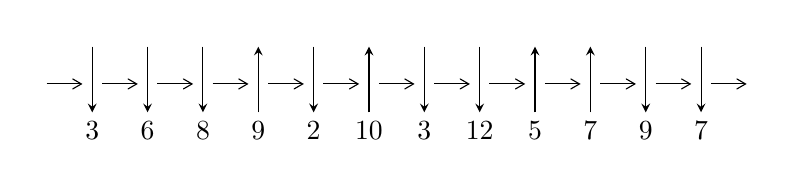
\begin{tikzpicture}[x=20pt, y=17pt]
	% nodes
	\node (C0) at (0, 0) {};
	\node (C1) at (1, 0) {};
	\node (C1U) at (1, +1) {};
	\node (C1D) at (1, -1) {3};

	\node (C2) at (2, 0) {};
	\node (C2U) at (2, +1) {};
	\node (C2D) at (2, -1) {6};

	\node (C3) at (3, 0) {};
	\node (C3U) at (3, +1) {};
	\node (C3D) at (3, -1) {8};

	\node (C4) at (4, 0) {};
	\node (C4U) at (4, +1) {};
	\node (C4D) at (4, -1) {9};

	\node (C5) at (5, 0) {};
	\node (C5U) at (5, +1) {};
	\node (C5D) at (5, -1) {2};

	\node (C6) at (6, 0) {};
	\node (C6U) at (6, +1) {};
	\node (C6D) at (6, -1) {10};

	\node (C7) at (7, 0) {};
	\node (C7U) at (7, +1) {};
	\node (C7D) at (7, -1) {3};

	\node (C8) at (8, 0) {};
	\node (C8U) at (8, +1) {};
	\node (C8D) at (8, -1) {12};

	\node (C9) at (9, 0) {};
	\node (C9U) at (9, +1) {};
	\node (C9D) at (9, -1) {5};

	\node (C10) at (10, 0) {};
	\node (C10U) at (10, +1) {};
	\node (C10D) at (10, -1) {7};

	\node (C11) at (11, 0) {};
	\node (C11U) at (11, +1) {};
	\node (C11D) at (11, -1) {9};

	\node (C12) at (12, 0) {};
	\node (C12U) at (12, +1) {};
	\node (C12D) at (12, -1) {7};
	\node (C13) at (13, 0) {};

	% arrows
	\draw[->,>={angle 60}]
	(C0) edge (C1) (C1) edge (C2) (C2) edge (C3) (C3) edge (C4) (C4) edge (C5) (C5) edge (C6) (C6) edge (C7) (C7) edge (C8) (C8) edge (C9) (C9) edge (C10) (C10) edge (C11) (C11) edge (C12) (C12) edge (C13) ;	\draw[->,>=stealth]
	(C1U) edge (C1D) (C2U) edge (C2D) (C3U) edge (C3D) (C4D) edge (C4U) (C5U) edge (C5D) (C6D) edge (C6U) (C7U) edge (C7D) (C8U) edge (C8D) (C9D) edge (C9U) (C10D) edge (C10U) (C11U) edge (C11D) (C12U) edge (C12D) ;
	\end{tikzpicture} \\
\hhline{~~} \\& 
\textbf{Solving Sequence} \\ \cline{2-2} 
 &
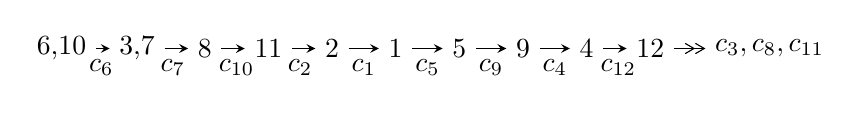
\begin{tikzpicture}[x=23pt, y=7pt]
	% node
	\node (A0) at (-1/8, 0) {6,10};
	\node (A1) at (17/16, 0) {3,7};
	\node (A2) at (17/8, 0) {8};
	\node (A3) at (25/8, 0) {11};
	\node (A4) at (33/8, 0) {2};
	\node (A5) at (41/8, 0) {1};
	\node (A6) at (49/8, 0) {5};
	\node (A7) at (57/8, 0) {9};
	\node (A8) at (65/8, 0) {4};
	\node (A9) at (73/8, 0) {12};
	\node (C1) at (1/2, -1) {$c_{6}$};
	\node (C2) at (13/8, -1) {$c_{7}$};
	\node (C3) at (21/8, -1) {$c_{10}$};
	\node (C4) at (29/8, -1) {$c_{2}$};
	\node (C5) at (37/8, -1) {$c_{1}$};
	\node (C6) at (45/8, -1) {$c_{5}$};
	\node (C7) at (53/8, -1) {$c_{9}$};
	\node (C8) at (61/8, -1) {$c_{4}$};
	\node (C9) at (69/8, -1) {$c_{12}$};
	\node (A10) at (11, 0) {$c_{3},c_{8},c_{11}$};

	% edge
	\draw[->,>=stealth]	
	(A0) edge (A1) (A1) edge (A2) (A2) edge (A3) (A3) edge (A4) (A4) edge (A5) (A5) edge (A6) (A6) edge (A7) (A7) edge (A8) (A8) edge (A9) ;
	\draw[->>,>={angle 60}]	
	(A9) edge (A10);
\end{tikzpicture} \\ 

\end{tabular} \\

\footnotetext{
The image of knot diagram is generated by the software ``\textbf{Draw programme}" developed by Andrew Bartholomew(\url{http://www.layer8.co.uk/maths/draw/index.htm\#Running-draw}), where we modified some parts for our purpose(\url{https://github.com/CATsTAILs/LinksPainter}).
}\phantom \\ \newline 
\centering \textbf{Ideals for irreducible components\footnotemark of $X_{\text{par}}$} 
 
\begin{align*}
I^u_{1}&=\langle 
-1.29866\times10^{170} u^{65}-1.30524\times10^{169} u^{64}+\cdots+2.37368\times10^{172} b+1.61064\times10^{172},\\
\phantom{I^u_{1}}&\phantom{= \langle  }-1.42092\times10^{172} u^{65}-6.96969\times10^{171} u^{64}+\cdots+1.40047\times10^{174} a-5.29249\times10^{174},\\
\phantom{I^u_{1}}&\phantom{= \langle  }u^{66}- u^{65}+\cdots-283 u-59\rangle \\
I^u_{2}&=\langle 
-547107839 u^{20}+650340830 u^{19}+\cdots+16127515 b+671904942,\\
\phantom{I^u_{2}}&\phantom{= \langle  }1292670203 u^{20}-1531668600 u^{19}+\cdots+16127515 a-1597251904,\;u^{21}-2 u^{20}+\cdots-2 u+1\rangle \\
\\
\end{align*}
\raggedright * 2 irreducible components of $\dim_{\mathbb{C}}=0$, with total 87 representations.\\
\footnotetext{All coefficients of polynomials are rational numbers. But the coefficients are sometimes approximated in decimal forms when there is not enough margin.}
\newpage
\renewcommand{\arraystretch}{1}
\centering \section*{I. $I^u_{1}= \langle -1.30\times10^{170} u^{65}-1.31\times10^{169} u^{64}+\cdots+2.37\times10^{172} b+1.61\times10^{172},\;-1.42\times10^{172} u^{65}-6.97\times10^{171} u^{64}+\cdots+1.40\times10^{174} a-5.29\times10^{174},\;u^{66}- u^{65}+\cdots-283 u-59 \rangle$}
\flushleft \textbf{(i) Arc colorings}\\
\begin{tabular}{m{7pt} m{180pt} m{7pt} m{180pt} }
\flushright $a_{6}=$&$\begin{pmatrix}1\\0\end{pmatrix}$ \\
\flushright $a_{10}=$&$\begin{pmatrix}0\\u\end{pmatrix}$ \\
\flushright $a_{3}=$&$\begin{pmatrix}0.0101460 u^{65}+0.00497667 u^{64}+\cdots-6.90436 u+3.77907\\0.00547109 u^{65}+0.000549881 u^{64}+\cdots+0.213003 u-0.678540\end{pmatrix}$ \\
\flushright $a_{7}=$&$\begin{pmatrix}1\\- u^2\end{pmatrix}$ \\
\flushright $a_{8}=$&$\begin{pmatrix}-0.0371999 u^{65}+0.000132037 u^{64}+\cdots-10.9635 u-4.32444\\0.00558096 u^{65}-0.00149963 u^{64}+\cdots+2.52802 u+0.980850\end{pmatrix}$ \\
\flushright $a_{11}=$&$\begin{pmatrix}u\\- u^3+u\end{pmatrix}$ \\
\flushright $a_{2}=$&$\begin{pmatrix}0.0156171 u^{65}+0.00552655 u^{64}+\cdots-6.69135 u+3.10053\\0.00547109 u^{65}+0.000549881 u^{64}+\cdots+0.213003 u-0.678540\end{pmatrix}$ \\
\flushright $a_{1}=$&$\begin{pmatrix}0.0130843 u^{65}-0.00173031 u^{64}+\cdots+1.28588 u+1.21472\\-0.00482668 u^{65}-0.00301544 u^{64}+\cdots+1.23112 u-0.215116\end{pmatrix}$ \\
\flushright $a_{5}=$&$\begin{pmatrix}-0.00412372 u^{65}+0.0123233 u^{64}+\cdots-10.8977 u+2.49609\\-0.0176584 u^{65}+0.00749844 u^{64}+\cdots-8.52232 u-2.06406\end{pmatrix}$ \\
\flushright $a_{9}=$&$\begin{pmatrix}0.0252026 u^{65}+0.00297306 u^{64}+\cdots+2.79443 u+2.86901\\-0.00121735 u^{65}+0.00691108 u^{64}+\cdots-4.53204 u-1.11595\end{pmatrix}$ \\
\flushright $a_{4}=$&$\begin{pmatrix}-0.0725476 u^{65}+0.0237047 u^{64}+\cdots-35.1307 u-2.94708\\-0.0312738 u^{65}+0.00209774 u^{64}+\cdots-8.36009 u-1.96671\end{pmatrix}$ \\
\flushright $a_{12}=$&$\begin{pmatrix}0.0148679 u^{65}-0.00641855 u^{64}+\cdots+6.50217 u+1.66949\\-0.000909781 u^{65}-0.00295631 u^{64}+\cdots+1.94792 u-0.0437386\end{pmatrix}$\\&\end{tabular}
\flushleft \textbf{(ii) Obstruction class $= -1$}\\~\\
\flushleft \textbf{(iii) Cusp Shapes $= 0.0549937 u^{65}+0.0239803 u^{64}+\cdots-1.32112 u-6.19761$}\\~\\
\newpage\renewcommand{\arraystretch}{1}
\flushleft \textbf{(iv) u-Polynomials at the component}\newline \\
\begin{tabular}{m{50pt}|m{274pt}}
Crossings & \hspace{64pt}u-Polynomials at each crossing \\
\hline $$\begin{aligned}c_{1}\end{aligned}$$&$\begin{aligned}
&u^{66}+38 u^{65}+\cdots-20 u+1
\end{aligned}$\\
\hline $$\begin{aligned}c_{2},c_{5}\end{aligned}$$&$\begin{aligned}
&u^{66}+2 u^{65}+\cdots+10 u^2+1
\end{aligned}$\\
\hline $$\begin{aligned}c_{3},c_{7}\end{aligned}$$&$\begin{aligned}
&u^{66}- u^{65}+\cdots-599 u-59
\end{aligned}$\\
\hline $$\begin{aligned}c_{4},c_{9}\end{aligned}$$&$\begin{aligned}
&u^{66}+u^{65}+\cdots+1920 u-1088
\end{aligned}$\\
\hline $$\begin{aligned}c_{6},c_{10}\end{aligned}$$&$\begin{aligned}
&u^{66}- u^{65}+\cdots-283 u-59
\end{aligned}$\\
\hline $$\begin{aligned}c_{8},c_{11}\end{aligned}$$&$\begin{aligned}
&u^{66}-2 u^{65}+\cdots-13 u+1
\end{aligned}$\\
\hline $$\begin{aligned}c_{12}\end{aligned}$$&$\begin{aligned}
&u^{66}+2 u^{65}+\cdots+2893677 u+899893
\end{aligned}$\\
\hline
\end{tabular}\\~\\
\newpage\renewcommand{\arraystretch}{1}
\flushleft \textbf{(v) Riley Polynomials at the component}\newline \\
\begin{tabular}{m{50pt}|m{274pt}}
Crossings & \hspace{64pt}Riley Polynomials at each crossing \\
\hline $$\begin{aligned}c_{1}\end{aligned}$$&$\begin{aligned}
&y^{66}-6 y^{65}+\cdots+88 y+1
\end{aligned}$\\
\hline $$\begin{aligned}c_{2},c_{5}\end{aligned}$$&$\begin{aligned}
&y^{66}-38 y^{65}+\cdots+20 y+1
\end{aligned}$\\
\hline $$\begin{aligned}c_{3},c_{7}\end{aligned}$$&$\begin{aligned}
&y^{66}-71 y^{65}+\cdots-683301 y+3481
\end{aligned}$\\
\hline $$\begin{aligned}c_{4},c_{9}\end{aligned}$$&$\begin{aligned}
&y^{66}-27 y^{65}+\cdots-23148544 y+1183744
\end{aligned}$\\
\hline $$\begin{aligned}c_{6},c_{10}\end{aligned}$$&$\begin{aligned}
&y^{66}-29 y^{65}+\cdots-212367 y+3481
\end{aligned}$\\
\hline $$\begin{aligned}c_{8},c_{11}\end{aligned}$$&$\begin{aligned}
&y^{66}+18 y^{65}+\cdots-11 y+1
\end{aligned}$\\
\hline $$\begin{aligned}c_{12}\end{aligned}$$&$\begin{aligned}
&y^{66}-78 y^{65}+\cdots-13342381349441 y+809807411449
\end{aligned}$\\
\hline
\end{tabular}\\~\\
\newpage\flushleft \textbf{(vi) Complex Volumes and Cusp Shapes}
$$\begin{array}{c|c|c}  
\text{Solutions to }I^u_{1}& \I (\text{vol} + \sqrt{-1}CS) & \text{Cusp shape}\\
 \hline 
\begin{aligned}
u &= -1.009630 + 0.086875 I \\
a &= -0.865155 + 0.695569 I \\
b &= \phantom{-}0.646730 - 0.858274 I\end{aligned}
 & \phantom{-}6.63058 + 2.08531 I & \phantom{-}4.22354 - 2.28056 I \\ \hline\begin{aligned}
u &= -1.009630 - 0.086875 I \\
a &= -0.865155 - 0.695569 I \\
b &= \phantom{-}0.646730 + 0.858274 I\end{aligned}
 & \phantom{-}6.63058 - 2.08531 I & \phantom{-}4.22354 + 2.28056 I \\ \hline\begin{aligned}
u &= -0.630698 + 0.819545 I \\
a &= -1.08564 + 1.29025 I \\
b &= -0.145705 - 0.660230 I\end{aligned}
 & -5.32397 - 3.61939 I & -3.35802 + 3.00391 I \\ \hline\begin{aligned}
u &= -0.630698 - 0.819545 I \\
a &= -1.08564 - 1.29025 I \\
b &= -0.145705 + 0.660230 I\end{aligned}
 & -5.32397 + 3.61939 I & -3.35802 - 3.00391 I \\ \hline\begin{aligned}
u &= \phantom{-}0.855944 + 0.373732 I \\
a &= \phantom{-}0.776245 + 1.037920 I \\
b &= -0.979060 - 0.922126 I\end{aligned}
 & \phantom{-}3.16003 - 1.29810 I & -3.61685 - 1.27981 I \\ \hline\begin{aligned}
u &= \phantom{-}0.855944 - 0.373732 I \\
a &= \phantom{-}0.776245 - 1.037920 I \\
b &= -0.979060 + 0.922126 I\end{aligned}
 & \phantom{-}3.16003 + 1.29810 I & -3.61685 + 1.27981 I \\ \hline\begin{aligned}
u &= \phantom{-}0.919240 + 0.154057 I \\
a &= -0.06475 - 2.48944 I \\
b &= -0.959746 + 0.202331 I\end{aligned}
 & -0.086654 + 0.709749 I & \phantom{-}14.6199 + 25.0798 I \\ \hline\begin{aligned}
u &= \phantom{-}0.919240 - 0.154057 I \\
a &= -0.06475 + 2.48944 I \\
b &= -0.959746 - 0.202331 I\end{aligned}
 & -0.086654 - 0.709749 I & \phantom{-}14.6199 - 25.0798 I \\ \hline\begin{aligned}
u &= \phantom{-}0.916029 + 0.574839 I \\
a &= \phantom{-}0.02130 - 1.84018 I \\
b &= -0.915687 + 0.841121 I\end{aligned}
 & \phantom{-}3.26731 + 5.19167 I & -4.00000 - 5.91453 I \\ \hline\begin{aligned}
u &= \phantom{-}0.916029 - 0.574839 I \\
a &= \phantom{-}0.02130 + 1.84018 I \\
b &= -0.915687 - 0.841121 I\end{aligned}
 & \phantom{-}3.26731 - 5.19167 I & -4.00000 + 5.91453 I\\
 \hline 
 \end{array}$$\newpage$$\begin{array}{c|c|c}  
\text{Solutions to }I^u_{1}& \I (\text{vol} + \sqrt{-1}CS) & \text{Cusp shape}\\
 \hline 
\begin{aligned}
u &= -0.173418 + 1.076000 I \\
a &= \phantom{-}0.606519 + 0.088557 I \\
b &= \phantom{-}0.974893 - 0.350221 I\end{aligned}
 & -2.26147 + 3.75022 I & -5.56446 - 6.85194 I \\ \hline\begin{aligned}
u &= -0.173418 - 1.076000 I \\
a &= \phantom{-}0.606519 - 0.088557 I \\
b &= \phantom{-}0.974893 + 0.350221 I\end{aligned}
 & -2.26147 - 3.75022 I & -5.56446 + 6.85194 I \\ \hline\begin{aligned}
u &= -0.519698 + 0.732621 I \\
a &= -0.109977 + 0.297576 I \\
b &= \phantom{-}1.47718 - 0.21621 I\end{aligned}
 & -10.75900 + 2.41313 I & -9.03127 + 1.73650 I \\ \hline\begin{aligned}
u &= -0.519698 - 0.732621 I \\
a &= -0.109977 - 0.297576 I \\
b &= \phantom{-}1.47718 + 0.21621 I\end{aligned}
 & -10.75900 - 2.41313 I & -9.03127 - 1.73650 I \\ \hline\begin{aligned}
u &= -0.749346 + 0.349951 I \\
a &= \phantom{-}0.55197 - 1.77976 I \\
b &= \phantom{-}1.059490 + 0.777077 I\end{aligned}
 & \phantom{-}5.42275 - 4.01479 I & \phantom{-}2.47646 + 2.55070 I \\ \hline\begin{aligned}
u &= -0.749346 - 0.349951 I \\
a &= \phantom{-}0.55197 + 1.77976 I \\
b &= \phantom{-}1.059490 - 0.777077 I\end{aligned}
 & \phantom{-}5.42275 + 4.01479 I & \phantom{-}2.47646 - 2.55070 I \\ \hline\begin{aligned}
u &= \phantom{-}1.067390 + 0.520714 I \\
a &= -0.98150 + 1.66983 I \\
b &= \phantom{-}1.164360 - 0.472130 I\end{aligned}
 & -8.03045 + 0.12830 I & \phantom{-0.000000 } 0 \\ \hline\begin{aligned}
u &= \phantom{-}1.067390 - 0.520714 I \\
a &= -0.98150 - 1.66983 I \\
b &= \phantom{-}1.164360 + 0.472130 I\end{aligned}
 & -8.03045 - 0.12830 I & \phantom{-0.000000 } 0 \\ \hline\begin{aligned}
u &= -0.969229 + 0.691515 I \\
a &= \phantom{-}0.445965 - 1.042750 I \\
b &= -0.375558 + 1.052890 I\end{aligned}
 & -4.37518 - 1.96161 I & \phantom{-0.000000 } 0 \\ \hline\begin{aligned}
u &= -0.969229 - 0.691515 I \\
a &= \phantom{-}0.445965 + 1.042750 I \\
b &= -0.375558 - 1.052890 I\end{aligned}
 & -4.37518 + 1.96161 I & \phantom{-0.000000 } 0\\
 \hline 
 \end{array}$$\newpage$$\begin{array}{c|c|c}  
\text{Solutions to }I^u_{1}& \I (\text{vol} + \sqrt{-1}CS) & \text{Cusp shape}\\
 \hline 
\begin{aligned}
u &= \phantom{-}0.702254 + 0.396363 I \\
a &= -0.370907 - 0.419474 I \\
b &= \phantom{-}1.64825 + 0.27071 I\end{aligned}
 & -9.41079 + 3.73475 I & -1.97764 - 7.57060 I \\ \hline\begin{aligned}
u &= \phantom{-}0.702254 - 0.396363 I \\
a &= -0.370907 + 0.419474 I \\
b &= \phantom{-}1.64825 - 0.27071 I\end{aligned}
 & -9.41079 - 3.73475 I & -1.97764 + 7.57060 I \\ \hline\begin{aligned}
u &= \phantom{-}0.189571 + 0.774061 I \\
a &= -2.16201 - 0.76177 I \\
b &= -0.048717 + 0.448000 I\end{aligned}
 & -5.12953 - 3.97226 I & -2.53620 + 0.67549 I \\ \hline\begin{aligned}
u &= \phantom{-}0.189571 - 0.774061 I \\
a &= -2.16201 + 0.76177 I \\
b &= -0.048717 - 0.448000 I\end{aligned}
 & -5.12953 + 3.97226 I & -2.53620 - 0.67549 I \\ \hline\begin{aligned}
u &= -1.199090 + 0.103811 I \\
a &= \phantom{-}0.026151 + 0.873772 I \\
b &= -1.145820 - 0.448707 I\end{aligned}
 & \phantom{-}0.701365 + 0.560290 I & \phantom{-0.000000 } 0 \\ \hline\begin{aligned}
u &= -1.199090 - 0.103811 I \\
a &= \phantom{-}0.026151 - 0.873772 I \\
b &= -1.145820 + 0.448707 I\end{aligned}
 & \phantom{-}0.701365 - 0.560290 I & \phantom{-0.000000 } 0 \\ \hline\begin{aligned}
u &= -0.855896 + 0.851844 I \\
a &= -0.377073 + 0.226573 I \\
b &= -1.193960 - 0.293229 I\end{aligned}
 & \phantom{-}1.14814 - 4.23169 I & \phantom{-0.000000 } 0 \\ \hline\begin{aligned}
u &= -0.855896 - 0.851844 I \\
a &= -0.377073 - 0.226573 I \\
b &= -1.193960 + 0.293229 I\end{aligned}
 & \phantom{-}1.14814 + 4.23169 I & \phantom{-0.000000 } 0 \\ \hline\begin{aligned}
u &= -0.588541 + 0.473255 I \\
a &= \phantom{-}0.03657 + 2.05711 I \\
b &= -0.918831 - 0.419709 I\end{aligned}
 & -1.84865 - 1.55160 I & -9.86951 + 3.77741 I \\ \hline\begin{aligned}
u &= -0.588541 - 0.473255 I \\
a &= \phantom{-}0.03657 - 2.05711 I \\
b &= -0.918831 + 0.419709 I\end{aligned}
 & -1.84865 + 1.55160 I & -9.86951 - 3.77741 I\\
 \hline 
 \end{array}$$\newpage$$\begin{array}{c|c|c}  
\text{Solutions to }I^u_{1}& \I (\text{vol} + \sqrt{-1}CS) & \text{Cusp shape}\\
 \hline 
\begin{aligned}
u &= \phantom{-}0.583231 + 1.105720 I \\
a &= \phantom{-}0.365461 + 0.166066 I \\
b &= \phantom{-}0.875973 + 0.156748 I\end{aligned}
 & -1.25973 + 1.60946 I & \phantom{-0.000000 } 0 \\ \hline\begin{aligned}
u &= \phantom{-}0.583231 - 1.105720 I \\
a &= \phantom{-}0.365461 - 0.166066 I \\
b &= \phantom{-}0.875973 - 0.156748 I\end{aligned}
 & -1.25973 - 1.60946 I & \phantom{-0.000000 } 0 \\ \hline\begin{aligned}
u &= \phantom{-}1.26247\phantom{ +0.000000I} \\
a &= \phantom{-}1.73937\phantom{ +0.000000I} \\
b &= -0.819691\phantom{ +0.000000I}\end{aligned}
 & \phantom{-}0.936733\phantom{ +0.000000I} & \phantom{-0.000000 } 0 \\ \hline\begin{aligned}
u &= \phantom{-}0.678975 + 0.254457 I \\
a &= -1.38925 - 0.87609 I \\
b &= -1.140560 + 0.239727 I\end{aligned}
 & -0.962746 + 1.013270 I & -8.93256 + 2.66135 I \\ \hline\begin{aligned}
u &= \phantom{-}0.678975 - 0.254457 I \\
a &= -1.38925 + 0.87609 I \\
b &= -1.140560 - 0.239727 I\end{aligned}
 & -0.962746 - 1.013270 I & -8.93256 - 2.66135 I \\ \hline\begin{aligned}
u &= \phantom{-}1.198670 + 0.480794 I \\
a &= -0.123627 - 0.483725 I \\
b &= \phantom{-}0.438626 + 0.674148 I\end{aligned}
 & \phantom{-}3.38567 + 1.03176 I & \phantom{-0.000000 } 0 \\ \hline\begin{aligned}
u &= \phantom{-}1.198670 - 0.480794 I \\
a &= -0.123627 + 0.483725 I \\
b &= \phantom{-}0.438626 - 0.674148 I\end{aligned}
 & \phantom{-}3.38567 - 1.03176 I & \phantom{-0.000000 } 0 \\ \hline\begin{aligned}
u &= -1.140890 + 0.605827 I \\
a &= -0.62705 - 1.69841 I \\
b &= \phantom{-}1.184480 + 0.438695 I\end{aligned}
 & -8.77795 - 7.59235 I & \phantom{-0.000000 } 0 \\ \hline\begin{aligned}
u &= -1.140890 - 0.605827 I \\
a &= -0.62705 + 1.69841 I \\
b &= \phantom{-}1.184480 - 0.438695 I\end{aligned}
 & -8.77795 + 7.59235 I & \phantom{-0.000000 } 0 \\ \hline\begin{aligned}
u &= \phantom{-}1.147170 + 0.619204 I \\
a &= \phantom{-}0.319998 + 1.132160 I \\
b &= -0.308780 - 1.182400 I\end{aligned}
 & -2.68437 + 9.27943 I & \phantom{-0.000000 } 0\\
 \hline 
 \end{array}$$\newpage$$\begin{array}{c|c|c}  
\text{Solutions to }I^u_{1}& \I (\text{vol} + \sqrt{-1}CS) & \text{Cusp shape}\\
 \hline 
\begin{aligned}
u &= \phantom{-}1.147170 - 0.619204 I \\
a &= \phantom{-}0.319998 - 1.132160 I \\
b &= -0.308780 + 1.182400 I\end{aligned}
 & -2.68437 - 9.27943 I & \phantom{-0.000000 } 0 \\ \hline\begin{aligned}
u &= \phantom{-}1.297790 + 0.269866 I \\
a &= -0.049488 - 0.712548 I \\
b &= \phantom{-}0.375452 + 0.619653 I\end{aligned}
 & \phantom{-}3.28651 + 0.70632 I & \phantom{-0.000000 } 0 \\ \hline\begin{aligned}
u &= \phantom{-}1.297790 - 0.269866 I \\
a &= -0.049488 + 0.712548 I \\
b &= \phantom{-}0.375452 - 0.619653 I\end{aligned}
 & \phantom{-}3.28651 - 0.70632 I & \phantom{-0.000000 } 0 \\ \hline\begin{aligned}
u &= -1.306810 + 0.303581 I \\
a &= -0.254876 + 0.950359 I \\
b &= \phantom{-}0.155440 - 0.803337 I\end{aligned}
 & \phantom{-}4.37101 - 4.54876 I & \phantom{-0.000000 } 0 \\ \hline\begin{aligned}
u &= -1.306810 - 0.303581 I \\
a &= -0.254876 - 0.950359 I \\
b &= \phantom{-}0.155440 + 0.803337 I\end{aligned}
 & \phantom{-}4.37101 + 4.54876 I & \phantom{-0.000000 } 0 \\ \hline\begin{aligned}
u &= -0.792328 + 1.127230 I \\
a &= \phantom{-}0.245968 - 0.148562 I \\
b &= -1.193740 + 0.508031 I\end{aligned}
 & -8.28883 + 1.02130 I & \phantom{-0.000000 } 0 \\ \hline\begin{aligned}
u &= -0.792328 - 1.127230 I \\
a &= \phantom{-}0.245968 + 0.148562 I \\
b &= -1.193740 - 0.508031 I\end{aligned}
 & -8.28883 - 1.02130 I & \phantom{-0.000000 } 0 \\ \hline\begin{aligned}
u &= -1.269320 + 0.570574 I \\
a &= \phantom{-}0.100258 - 1.297270 I \\
b &= \phantom{-}1.217640 + 0.524719 I\end{aligned}
 & \phantom{-}1.20353 - 9.50394 I & \phantom{-0.000000 } 0 \\ \hline\begin{aligned}
u &= -1.269320 - 0.570574 I \\
a &= \phantom{-}0.100258 + 1.297270 I \\
b &= \phantom{-}1.217640 - 0.524719 I\end{aligned}
 & \phantom{-}1.20353 + 9.50394 I & \phantom{-0.000000 } 0 \\ \hline\begin{aligned}
u &= \phantom{-}0.98914 + 1.01218 I \\
a &= \phantom{-}0.405389 + 0.898557 I \\
b &= \phantom{-}1.065930 - 0.564917 I\end{aligned}
 & \phantom{-}1.55388 + 5.84749 I & \phantom{-0.000000 } 0\\
 \hline 
 \end{array}$$\newpage$$\begin{array}{c|c|c}  
\text{Solutions to }I^u_{1}& \I (\text{vol} + \sqrt{-1}CS) & \text{Cusp shape}\\
 \hline 
\begin{aligned}
u &= \phantom{-}0.98914 - 1.01218 I \\
a &= \phantom{-}0.405389 - 0.898557 I \\
b &= \phantom{-}1.065930 + 0.564917 I\end{aligned}
 & \phantom{-}1.55388 - 5.84749 I & \phantom{-0.000000 } 0 \\ \hline\begin{aligned}
u &= -1.14794 + 0.86562 I \\
a &= -0.01851 + 1.44202 I \\
b &= -1.23555 - 0.69019 I\end{aligned}
 & -7.02539 - 8.25526 I & \phantom{-0.000000 } 0 \\ \hline\begin{aligned}
u &= -1.14794 - 0.86562 I \\
a &= -0.01851 - 1.44202 I \\
b &= -1.23555 + 0.69019 I\end{aligned}
 & -7.02539 + 8.25526 I & \phantom{-0.000000 } 0 \\ \hline\begin{aligned}
u &= \phantom{-}0.137966 + 0.528220 I \\
a &= \phantom{-}0.796178 - 0.216051 I \\
b &= -0.031272 + 0.313358 I\end{aligned}
 & -0.101260 + 1.177890 I & -1.60509 - 5.48121 I \\ \hline\begin{aligned}
u &= \phantom{-}0.137966 - 0.528220 I \\
a &= \phantom{-}0.796178 + 0.216051 I \\
b &= -0.031272 - 0.313358 I\end{aligned}
 & -0.101260 - 1.177890 I & -1.60509 + 5.48121 I \\ \hline\begin{aligned}
u &= \phantom{-}0.020560 + 0.528328 I \\
a &= -4.29255 - 0.39915 I \\
b &= \phantom{-}0.176919 + 0.209119 I\end{aligned}
 & -5.14008 - 3.94973 I & \phantom{-}0.643204 - 0.090602 I \\ \hline\begin{aligned}
u &= \phantom{-}0.020560 - 0.528328 I \\
a &= -4.29255 + 0.39915 I \\
b &= \phantom{-}0.176919 - 0.209119 I\end{aligned}
 & -5.14008 + 3.94973 I & \phantom{-}0.643204 + 0.090602 I \\ \hline\begin{aligned}
u &= \phantom{-}1.27921 + 0.73272 I \\
a &= \phantom{-}0.076111 + 1.032910 I \\
b &= \phantom{-}1.118870 - 0.498354 I\end{aligned}
 & \phantom{-}1.06224 + 5.14116 I & \phantom{-0.000000 } 0 \\ \hline\begin{aligned}
u &= \phantom{-}1.27921 - 0.73272 I \\
a &= \phantom{-}0.076111 - 1.032910 I \\
b &= \phantom{-}1.118870 + 0.498354 I\end{aligned}
 & \phantom{-}1.06224 - 5.14116 I & \phantom{-0.000000 } 0 \\ \hline\begin{aligned}
u &= \phantom{-}0.64925 + 1.38410 I \\
a &= \phantom{-}0.118590 + 0.092801 I \\
b &= -1.156150 - 0.470421 I\end{aligned}
 & -8.02803 - 8.05910 I & \phantom{-0.000000 } 0\\
 \hline 
 \end{array}$$\newpage$$\begin{array}{c|c|c}  
\text{Solutions to }I^u_{1}& \I (\text{vol} + \sqrt{-1}CS) & \text{Cusp shape}\\
 \hline 
\begin{aligned}
u &= \phantom{-}0.64925 - 1.38410 I \\
a &= \phantom{-}0.118590 - 0.092801 I \\
b &= -1.156150 + 0.470421 I\end{aligned}
 & -8.02803 + 8.05910 I & \phantom{-0.000000 } 0 \\ \hline\begin{aligned}
u &= \phantom{-}1.28691 + 0.85432 I \\
a &= \phantom{-}0.034457 - 1.326560 I \\
b &= -1.29162 + 0.68757 I\end{aligned}
 & -5.7819 + 15.8817 I & \phantom{-0.000000 } 0 \\ \hline\begin{aligned}
u &= \phantom{-}1.28691 - 0.85432 I \\
a &= \phantom{-}0.034457 + 1.326560 I \\
b &= -1.29162 - 0.68757 I\end{aligned}
 & -5.7819 - 15.8817 I & \phantom{-0.000000 } 0 \\ \hline\begin{aligned}
u &= -1.63204 + 0.55209 I \\
a &= \phantom{-}0.385181 + 0.448101 I \\
b &= -0.729629 + 0.000860 I\end{aligned}
 & \phantom{-}3.55115 - 2.82787 I & \phantom{-0.000000 } 0 \\ \hline\begin{aligned}
u &= -1.63204 - 0.55209 I \\
a &= \phantom{-}0.385181 - 0.448101 I \\
b &= -0.729629 - 0.000860 I\end{aligned}
 & \phantom{-}3.55115 + 2.82787 I & \phantom{-0.000000 } 0 \\ \hline\begin{aligned}
u &= -0.131285\phantom{ +0.000000I} \\
a &= \phantom{-}4.53665\phantom{ +0.000000I} \\
b &= -0.799964\phantom{ +0.000000I}\end{aligned}
 & -1.37349\phantom{ +0.000000I} & -6.68870\phantom{ +0.000000I}\\
 \hline 
 \end{array}$$\newpage\newpage\renewcommand{\arraystretch}{1}
\centering \section*{II. $I^u_{2}= \langle -5.47\times10^{8} u^{20}+6.50\times10^{8} u^{19}+\cdots+1.61\times10^{7} b+6.72\times10^{8},\;1.29\times10^{9} u^{20}-1.53\times10^{9} u^{19}+\cdots+1.61\times10^{7} a-1.60\times10^{9},\;u^{21}-2 u^{20}+\cdots-2 u+1 \rangle$}
\flushleft \textbf{(i) Arc colorings}\\
\begin{tabular}{m{7pt} m{180pt} m{7pt} m{180pt} }
\flushright $a_{6}=$&$\begin{pmatrix}1\\0\end{pmatrix}$ \\
\flushright $a_{10}=$&$\begin{pmatrix}0\\u\end{pmatrix}$ \\
\flushright $a_{3}=$&$\begin{pmatrix}-80.1531 u^{20}+94.9724 u^{19}+\cdots-77.1772 u+99.0389\\33.9239 u^{20}-40.3249 u^{19}+\cdots+33.3984 u-41.6620\end{pmatrix}$ \\
\flushright $a_{7}=$&$\begin{pmatrix}1\\- u^2\end{pmatrix}$ \\
\flushright $a_{8}=$&$\begin{pmatrix}89.2432 u^{20}-106.092 u^{19}+\cdots+85.7475 u-114.343\\-17.4567 u^{20}+21.6317 u^{19}+\cdots-15.1161 u+23.6718\end{pmatrix}$ \\
\flushright $a_{11}=$&$\begin{pmatrix}u\\- u^3+u\end{pmatrix}$ \\
\flushright $a_{2}=$&$\begin{pmatrix}-46.2292 u^{20}+54.6475 u^{19}+\cdots-43.7787 u+57.3769\\33.9239 u^{20}-40.3249 u^{19}+\cdots+33.3984 u-41.6620\end{pmatrix}$ \\
\flushright $a_{1}=$&$\begin{pmatrix}26.1717 u^{20}-31.1465 u^{19}+\cdots+27.5071 u-29.6074\\-89.8576 u^{20}+107.426 u^{19}+\cdots-86.4020 u+110.656\end{pmatrix}$ \\
\flushright $a_{5}=$&$\begin{pmatrix}-17.4567 u^{20}+20.6317 u^{19}+\cdots-17.1161 u+23.6718\\80.1961 u^{20}-95.9634 u^{19}+\cdots+74.8843 u-102.382\end{pmatrix}$ \\
\flushright $a_{9}=$&$\begin{pmatrix}-33.2945 u^{20}+41.0318 u^{19}+\cdots-30.7499 u+39.7364\\62.0383 u^{20}-74.4291 u^{19}+\cdots+62.2499 u-77.2800\end{pmatrix}$ \\
\flushright $a_{4}=$&$\begin{pmatrix}24.4461 u^{20}-28.8789 u^{19}+\cdots+22.7417 u-29.0227\\31.8485 u^{20}-37.6738 u^{19}+\cdots+32.8621 u-43.6846\end{pmatrix}$ \\
\flushright $a_{12}=$&$\begin{pmatrix}-46.8592 u^{20}+56.0635 u^{19}+\cdots-42.6727 u+59.8518\\-42.9984 u^{20}+51.3621 u^{19}+\cdots-41.7293 u+51.8043\end{pmatrix}$\\&\end{tabular}
\flushleft \textbf{(ii) Obstruction class $= 1$}\\~\\
\flushleft \textbf{(iii) Cusp Shapes $= -\frac{1978262081}{16127515} u^{20}+\frac{486999773}{3225503} u^{19}+\cdots-\frac{1665299122}{16127515} u+\frac{2329754158}{16127515}$}\\~\\
\newpage\renewcommand{\arraystretch}{1}
\flushleft \textbf{(iv) u-Polynomials at the component}\newline \\
\begin{tabular}{m{50pt}|m{274pt}}
Crossings & \hspace{64pt}u-Polynomials at each crossing \\
\hline $$\begin{aligned}c_{1}\end{aligned}$$&$\begin{aligned}
&u^{21}-13 u^{20}+\cdots+17 u-1
\end{aligned}$\\
\hline $$\begin{aligned}c_{2}\end{aligned}$$&$\begin{aligned}
&u^{21}+3 u^{20}+\cdots-3 u-1
\end{aligned}$\\
\hline $$\begin{aligned}c_{3}\end{aligned}$$&$\begin{aligned}
&u^{21}-9 u^{19}+\cdots-6 u+1
\end{aligned}$\\
\hline $$\begin{aligned}c_{4}\end{aligned}$$&$\begin{aligned}
&u^{21}-7 u^{19}+\cdots+9 u^2+1
\end{aligned}$\\
\hline $$\begin{aligned}c_{5}\end{aligned}$$&$\begin{aligned}
&u^{21}-3 u^{20}+\cdots-3 u+1
\end{aligned}$\\
\hline $$\begin{aligned}c_{6}\end{aligned}$$&$\begin{aligned}
&u^{21}-2 u^{20}+\cdots-2 u+1
\end{aligned}$\\
\hline $$\begin{aligned}c_{7}\end{aligned}$$&$\begin{aligned}
&u^{21}-9 u^{19}+\cdots-6 u-1
\end{aligned}$\\
\hline $$\begin{aligned}c_{8}\end{aligned}$$&$\begin{aligned}
&u^{21}-3 u^{20}+\cdots-4 u+1
\end{aligned}$\\
\hline $$\begin{aligned}c_{9}\end{aligned}$$&$\begin{aligned}
&u^{21}-7 u^{19}+\cdots-9 u^2-1
\end{aligned}$\\
\hline $$\begin{aligned}c_{10}\end{aligned}$$&$\begin{aligned}
&u^{21}+2 u^{20}+\cdots-2 u-1
\end{aligned}$\\
\hline $$\begin{aligned}c_{11}\end{aligned}$$&$\begin{aligned}
&u^{21}+3 u^{20}+\cdots-4 u-1
\end{aligned}$\\
\hline $$\begin{aligned}c_{12}\end{aligned}$$&$\begin{aligned}
&u^{21}- u^{20}+\cdots+12 u+1
\end{aligned}$\\
\hline
\end{tabular}\\~\\
\newpage\renewcommand{\arraystretch}{1}
\flushleft \textbf{(v) Riley Polynomials at the component}\newline \\
\begin{tabular}{m{50pt}|m{274pt}}
Crossings & \hspace{64pt}Riley Polynomials at each crossing \\
\hline $$\begin{aligned}c_{1}\end{aligned}$$&$\begin{aligned}
&y^{21}+3 y^{20}+\cdots+17 y-1
\end{aligned}$\\
\hline $$\begin{aligned}c_{2},c_{5}\end{aligned}$$&$\begin{aligned}
&y^{21}-13 y^{20}+\cdots+17 y-1
\end{aligned}$\\
\hline $$\begin{aligned}c_{3},c_{7}\end{aligned}$$&$\begin{aligned}
&y^{21}-18 y^{20}+\cdots+22 y-1
\end{aligned}$\\
\hline $$\begin{aligned}c_{4},c_{9}\end{aligned}$$&$\begin{aligned}
&y^{21}-14 y^{20}+\cdots-18 y-1
\end{aligned}$\\
\hline $$\begin{aligned}c_{6},c_{10}\end{aligned}$$&$\begin{aligned}
&y^{21}-12 y^{20}+\cdots-4 y-1
\end{aligned}$\\
\hline $$\begin{aligned}c_{8},c_{11}\end{aligned}$$&$\begin{aligned}
&y^{21}+15 y^{20}+\cdots-8 y-1
\end{aligned}$\\
\hline $$\begin{aligned}c_{12}\end{aligned}$$&$\begin{aligned}
&y^{21}+3 y^{20}+\cdots+26 y-1
\end{aligned}$\\
\hline
\end{tabular}\\~\\
\newpage\flushleft \textbf{(vi) Complex Volumes and Cusp Shapes}
$$\begin{array}{c|c|c}  
\text{Solutions to }I^u_{2}& \I (\text{vol} + \sqrt{-1}CS) & \text{Cusp shape}\\
 \hline 
\begin{aligned}
u &= -0.497705 + 0.914980 I \\
a &= -0.500009 + 0.376999 I \\
b &= -0.883156 - 0.078797 I\end{aligned}
 & -1.39865 - 2.19121 I & -5.26683 + 7.34066 I \\ \hline\begin{aligned}
u &= -0.497705 - 0.914980 I \\
a &= -0.500009 - 0.376999 I \\
b &= -0.883156 + 0.078797 I\end{aligned}
 & -1.39865 + 2.19121 I & -5.26683 - 7.34066 I \\ \hline\begin{aligned}
u &= -0.906547 + 0.120990 I \\
a &= -0.37152 + 1.92475 I \\
b &= -1.049690 - 0.261917 I\end{aligned}
 & -0.291019 - 0.766881 I & -12.9784 - 7.1305 I \\ \hline\begin{aligned}
u &= -0.906547 - 0.120990 I \\
a &= -0.37152 - 1.92475 I \\
b &= -1.049690 + 0.261917 I\end{aligned}
 & -0.291019 + 0.766881 I & -12.9784 + 7.1305 I \\ \hline\begin{aligned}
u &= -0.952688 + 0.665934 I \\
a &= \phantom{-}0.31948 - 1.54539 I \\
b &= \phantom{-}0.968691 + 0.804354 I\end{aligned}
 & \phantom{-}4.83291 - 5.48153 I & \phantom{-}0.61562 + 6.66233 I \\ \hline\begin{aligned}
u &= -0.952688 - 0.665934 I \\
a &= \phantom{-}0.31948 + 1.54539 I \\
b &= \phantom{-}0.968691 - 0.804354 I\end{aligned}
 & \phantom{-}4.83291 + 5.48153 I & \phantom{-}0.61562 - 6.66233 I \\ \hline\begin{aligned}
u &= -1.063450 + 0.512232 I \\
a &= -0.589209 + 0.637928 I \\
b &= \phantom{-}0.810459 - 0.843136 I\end{aligned}
 & \phantom{-}5.31654 + 0.66491 I & \phantom{-}0.415399 - 0.133048 I \\ \hline\begin{aligned}
u &= -1.063450 - 0.512232 I \\
a &= -0.589209 - 0.637928 I \\
b &= \phantom{-}0.810459 + 0.843136 I\end{aligned}
 & \phantom{-}5.31654 - 0.66491 I & \phantom{-}0.415399 + 0.133048 I \\ \hline\begin{aligned}
u &= \phantom{-}0.801649 + 0.001085 I \\
a &= \phantom{-}0.07947 - 1.82807 I \\
b &= -1.18975 + 0.76944 I\end{aligned}
 & \phantom{-}3.72958 + 2.65022 I & -0.33689 - 2.74170 I \\ \hline\begin{aligned}
u &= \phantom{-}0.801649 - 0.001085 I \\
a &= \phantom{-}0.07947 + 1.82807 I \\
b &= -1.18975 - 0.76944 I\end{aligned}
 & \phantom{-}3.72958 - 2.65022 I & -0.33689 + 2.74170 I\\
 \hline 
 \end{array}$$\newpage$$\begin{array}{c|c|c}  
\text{Solutions to }I^u_{2}& \I (\text{vol} + \sqrt{-1}CS) & \text{Cusp shape}\\
 \hline 
\begin{aligned}
u &= -1.19930\phantom{ +0.000000I} \\
a &= \phantom{-}1.40578\phantom{ +0.000000I} \\
b &= -0.550979\phantom{ +0.000000I}\end{aligned}
 & \phantom{-}1.39967\phantom{ +0.000000I} & -0.347370\phantom{ +0.000000I} \\ \hline\begin{aligned}
u &= \phantom{-}1.194170 + 0.163422 I \\
a &= \phantom{-}0.829774 - 1.015350 I \\
b &= -0.605623 + 0.779316 I\end{aligned}
 & \phantom{-}5.50035 + 3.30026 I & \phantom{-}1.09093 - 4.73816 I \\ \hline\begin{aligned}
u &= \phantom{-}1.194170 - 0.163422 I \\
a &= \phantom{-}0.829774 + 1.015350 I \\
b &= -0.605623 - 0.779316 I\end{aligned}
 & \phantom{-}5.50035 - 3.30026 I & \phantom{-}1.09093 + 4.73816 I \\ \hline\begin{aligned}
u &= \phantom{-}0.151730 + 0.674872 I \\
a &= \phantom{-}3.81452 + 0.99293 I \\
b &= \phantom{-}0.512186 - 0.147355 I\end{aligned}
 & -5.43869 + 4.12896 I & -19.9561 - 11.5234 I \\ \hline\begin{aligned}
u &= \phantom{-}0.151730 - 0.674872 I \\
a &= \phantom{-}3.81452 - 0.99293 I \\
b &= \phantom{-}0.512186 + 0.147355 I\end{aligned}
 & -5.43869 - 4.12896 I & -19.9561 + 11.5234 I \\ \hline\begin{aligned}
u &= \phantom{-}1.14383 + 1.06714 I \\
a &= \phantom{-}0.308798 + 0.748318 I \\
b &= \phantom{-}1.099210 - 0.485659 I\end{aligned}
 & \phantom{-}2.33435 + 5.94594 I & \phantom{-}3.05578 - 7.68621 I \\ \hline\begin{aligned}
u &= \phantom{-}1.14383 - 1.06714 I \\
a &= \phantom{-}0.308798 - 0.748318 I \\
b &= \phantom{-}1.099210 + 0.485659 I\end{aligned}
 & \phantom{-}2.33435 - 5.94594 I & \phantom{-}3.05578 + 7.68621 I \\ \hline\begin{aligned}
u &= \phantom{-}0.159929 + 0.360867 I \\
a &= -1.98062 + 0.02408 I \\
b &= \phantom{-}1.51366 + 0.09512 I\end{aligned}
 & -9.61177 + 2.97996 I & -4.78121 + 1.02692 I \\ \hline\begin{aligned}
u &= \phantom{-}0.159929 - 0.360867 I \\
a &= -1.98062 - 0.02408 I \\
b &= \phantom{-}1.51366 - 0.09512 I\end{aligned}
 & -9.61177 - 2.97996 I & -4.78121 - 1.02692 I \\ \hline\begin{aligned}
u &= \phantom{-}1.56873 + 0.63635 I \\
a &= -0.113575 - 0.201644 I \\
b &= \phantom{-}0.599496 + 0.365497 I\end{aligned}
 & \phantom{-}4.19616 + 2.23780 I & \phantom{-}2.81535 - 0.97091 I\\
 \hline 
 \end{array}$$\newpage$$\begin{array}{c|c|c}  
\text{Solutions to }I^u_{2}& \I (\text{vol} + \sqrt{-1}CS) & \text{Cusp shape}\\
 \hline 
\begin{aligned}
u &= \phantom{-}1.56873 - 0.63635 I \\
a &= -0.113575 + 0.201644 I \\
b &= \phantom{-}0.599496 - 0.365497 I\end{aligned}
 & \phantom{-}4.19616 - 2.23780 I & \phantom{-}2.81535 + 0.97091 I\\
 \hline 
 \end{array}$$\newpage
\newpage\renewcommand{\arraystretch}{1}
\centering \section*{ III. u-Polynomials}
\begin{tabular}{m{50pt}|m{274pt}}
Crossings & \hspace{64pt}u-Polynomials at each crossing \\
\hline $$\begin{aligned}c_{1}\end{aligned}$$&$\begin{aligned}
&(u^{21}-13 u^{20}+\cdots+17 u-1)(u^{66}+38 u^{65}+\cdots-20 u+1)
\end{aligned}$\\
\hline $$\begin{aligned}c_{2}\end{aligned}$$&$\begin{aligned}
&(u^{21}+3 u^{20}+\cdots-3 u-1)(u^{66}+2 u^{65}+\cdots+10 u^2+1)
\end{aligned}$\\
\hline $$\begin{aligned}c_{3}\end{aligned}$$&$\begin{aligned}
&(u^{21}-9 u^{19}+\cdots-6 u+1)(u^{66}- u^{65}+\cdots-599 u-59)
\end{aligned}$\\
\hline $$\begin{aligned}c_{4}\end{aligned}$$&$\begin{aligned}
&(u^{21}-7 u^{19}+\cdots+9 u^2+1)(u^{66}+u^{65}+\cdots+1920 u-1088)
\end{aligned}$\\
\hline $$\begin{aligned}c_{5}\end{aligned}$$&$\begin{aligned}
&(u^{21}-3 u^{20}+\cdots-3 u+1)(u^{66}+2 u^{65}+\cdots+10 u^2+1)
\end{aligned}$\\
\hline $$\begin{aligned}c_{6}\end{aligned}$$&$\begin{aligned}
&(u^{21}-2 u^{20}+\cdots-2 u+1)(u^{66}- u^{65}+\cdots-283 u-59)
\end{aligned}$\\
\hline $$\begin{aligned}c_{7}\end{aligned}$$&$\begin{aligned}
&(u^{21}-9 u^{19}+\cdots-6 u-1)(u^{66}- u^{65}+\cdots-599 u-59)
\end{aligned}$\\
\hline $$\begin{aligned}c_{8}\end{aligned}$$&$\begin{aligned}
&(u^{21}-3 u^{20}+\cdots-4 u+1)(u^{66}-2 u^{65}+\cdots-13 u+1)
\end{aligned}$\\
\hline $$\begin{aligned}c_{9}\end{aligned}$$&$\begin{aligned}
&(u^{21}-7 u^{19}+\cdots-9 u^2-1)(u^{66}+u^{65}+\cdots+1920 u-1088)
\end{aligned}$\\
\hline $$\begin{aligned}c_{10}\end{aligned}$$&$\begin{aligned}
&(u^{21}+2 u^{20}+\cdots-2 u-1)(u^{66}- u^{65}+\cdots-283 u-59)
\end{aligned}$\\
\hline $$\begin{aligned}c_{11}\end{aligned}$$&$\begin{aligned}
&(u^{21}+3 u^{20}+\cdots-4 u-1)(u^{66}-2 u^{65}+\cdots-13 u+1)
\end{aligned}$\\
\hline $$\begin{aligned}c_{12}\end{aligned}$$&$\begin{aligned}
&(u^{21}- u^{20}+\cdots+12 u+1)(u^{66}+2 u^{65}+\cdots+2893677 u+899893)
\end{aligned}$\\
\hline
\end{tabular}\newpage\renewcommand{\arraystretch}{1}
\centering \section*{ IV. Riley Polynomials}
\begin{tabular}{m{50pt}|m{274pt}}
Crossings & \hspace{64pt}Riley Polynomials at each crossing \\
\hline $$\begin{aligned}c_{1}\end{aligned}$$&$\begin{aligned}
&(y^{21}+3 y^{20}+\cdots+17 y-1)(y^{66}-6 y^{65}+\cdots+88 y+1)
\end{aligned}$\\
\hline $$\begin{aligned}c_{2},c_{5}\end{aligned}$$&$\begin{aligned}
&(y^{21}-13 y^{20}+\cdots+17 y-1)(y^{66}-38 y^{65}+\cdots+20 y+1)
\end{aligned}$\\
\hline $$\begin{aligned}c_{3},c_{7}\end{aligned}$$&$\begin{aligned}
&(y^{21}-18 y^{20}+\cdots+22 y-1)(y^{66}-71 y^{65}+\cdots-683301 y+3481)
\end{aligned}$\\
\hline $$\begin{aligned}c_{4},c_{9}\end{aligned}$$&$\begin{aligned}
&(y^{21}-14 y^{20}+\cdots-18 y-1)\\
&\cdot(y^{66}-27 y^{65}+\cdots-23148544 y+1183744)
\end{aligned}$\\
\hline $$\begin{aligned}c_{6},c_{10}\end{aligned}$$&$\begin{aligned}
&(y^{21}-12 y^{20}+\cdots-4 y-1)(y^{66}-29 y^{65}+\cdots-212367 y+3481)
\end{aligned}$\\
\hline $$\begin{aligned}c_{8},c_{11}\end{aligned}$$&$\begin{aligned}
&(y^{21}+15 y^{20}+\cdots-8 y-1)(y^{66}+18 y^{65}+\cdots-11 y+1)
\end{aligned}$\\
\hline $$\begin{aligned}c_{12}\end{aligned}$$&$\begin{aligned}
&(y^{21}+3 y^{20}+\cdots+26 y-1)\\
&\cdot(y^{66}-78 y^{65}+\cdots-13342381349441 y+809807411449)
\end{aligned}$\\
\hline
\end{tabular}
\vskip 2pc
\end{document}